\section{Foundational Concepts}
\label{sec:concepts}

\texttt{T-REX} is an adaptive, artificial intelligence based
controller and provides general framework for building reasoning
systems for real-world autonomous vehicles. At MBARI \texttt{T-REX} is
used for AUV control; another instantiation of the system is being
used for control of a terrestrial personal robot \cite{pr2,
  Meeussen:2010dn}. The development of \texttt{T-REX} has been
targeted at surveying a number of oceanographic features which are
dynamic and unpredictable spatio-temporally. Typically this requires
our AUVs to balance the goals of coverage spatially while
opportunistically following features of scientific interest and to do
so while being operationally aware of its own limitations in terms of
resources (typically the battery state of charge) and overall
proximity to other observational assets for obtaining scientific
ground-truth. We are therefore interested in representational
frameworks that allow robots to pursue long-term objectives while
choosing short-term gain and can gracefully deal with exogenous or
endogenous change.

To enable this responsiveness to external observations, the agent has
to be able to synthesize plans insitu and to re-plan. We use a
temporal constraint-based planner \eu with a demonstrated legacy of
having flown on NASA space missions \cite{jonsson00,bresina05,
  barreiro09}. Our autonomy architecture brings three key innovations
for AUV adaptation: the use of flexible plan representations,
compositional control with the use of partitioned networks and
off-line learning to inform insitu environmental state estimation. In
this section we detail some of the key concepts relevant to flexible
plan representation. Section \ref{sec:arch} has details the
\rx partitioned architecture and estimation driven vehicle
adaptation.

\subsection{The basics}
\label{sec:basics}

\eu uses a \emph{domain model} written in a declarative language
(NDDL: New Domain Description Language), together with initial
conditions and goals also specified in NDDL, to construct a set of
temporal relations that must be true at the start time. These models
include assertions about the physics of the vehicle, i.e how it
responds to external stimulus and internally driven goals. By
propagating these relations forward using Simple Temporal Networks
\cite{dechter91} and applying goal constraints, \eu can select a set
of conditions that should be true in the future, where some of these
conditions will correspond to actions the agent must take. The planner
can backtrack and try another path during search if a goal cannot be
reached while being capable of discarding unachievable goals.

Traditionally robot execution has relied on dispatching commands at
precise times. Such linear sequences of precisely timed commands give
no ability to adjust execution on the basis of sensory
information. Although some commands can issue tests on sensor
readings, these tests have the objective of verifying whether expected
execution conditions are occuring. If not, the state of the system is
declared off-nominal and execution of the sequence of commands is
interrupted. More recently, executives have been proposed and
implemented that significantly broaden the way robots can be commanded
\cite{mus98,alami:1998p820}. For example, the Remote Agent executive
interpreted a \textit{temporally flexible plan} which represents each
start time as a variable and contains an explicit network of bounded
delay constraints between such variables.

\begin{figure}[!t]
\centering
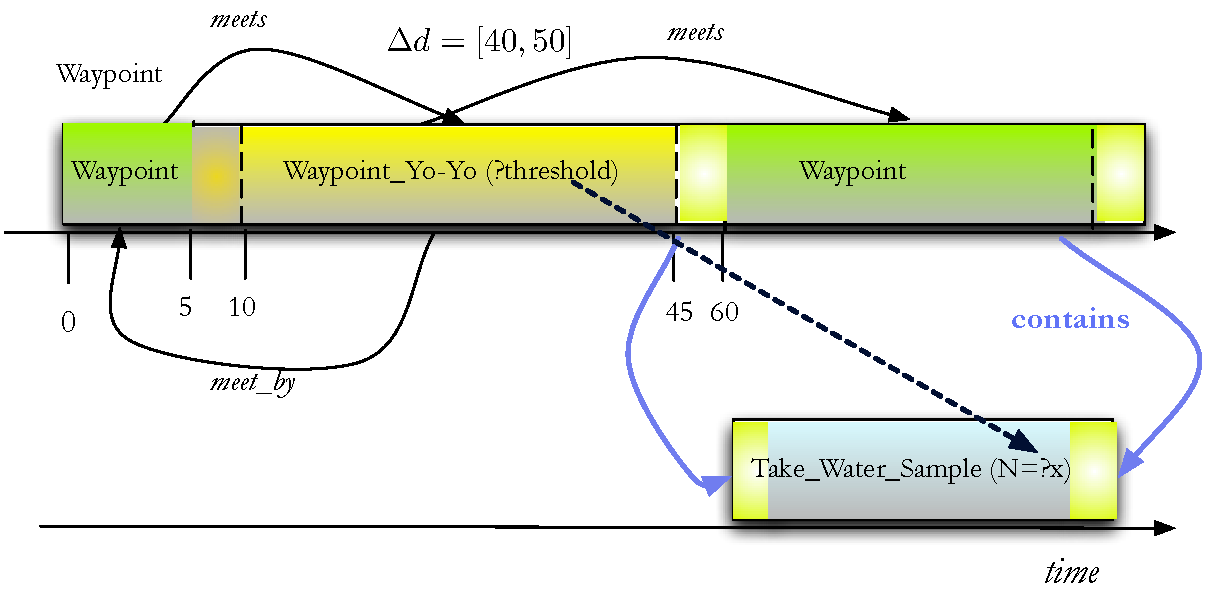
\includegraphics[scale=0.35]{figs/flexible-timelines.pdf}
\caption{\small Tokens with flexible temporal intervals and parametric
  constraints between tokens. This example shows the triggering of a
  water sampler based on a feature threshold while the vehicle
  Yo-Yo's. The \texttt{Waypoint\_Yo-Yo} token has a flexible duration,
  start \& end times.}
\label{fig:flex-timelines}
\vskip+0.1cm
\end{figure}

Unlike a traditional fixed time-tagged command sequences, such
flexible plans leave room for adaptation at execution time. When the
executive considers when to start a task, it propagates information
through the constraint network, computes a time bound for the
variable, selects an actual execution time within the bound, and
starts the task at that time. Temporally flexible plans therefore,
express a \textit{range of possible outcomes} of the robots
interaction with the environment within which the executive can elect
at run time the most appropriate one for the actual execution
conditions. The fact that constraints are explicitly represented
ensures that through constraint propagation the executive will respect
global limits expressed in the plan (e.g., don't start a task until a
certain condition has been satisfied but still satisfying some global
deadline). Such flexibility is critical when dealing with dynamic
ocean conditions where precise timing of a robotic action might be
indeterminate. Further, the advantage of flexibility can be contrasted
with the consequences of the intrinsic inflexibiliy of traditional
command sequences. Because they are inflexible, sequences must
necessarily be designed considering worst case scenarios.

\eu uses a \emph{state variable} representation to describe the
evolution of state over time. The instantiated history of such state
variable evolution over a temporal horizon we call \emph{timelines}
and which represent a single thread in the execution of a concurrent
system. At any given time each thread can execute a single procedure.
Thus each timeline consists of a sequence of procedures which
encapsulate and describe state evolution; we call these instantiated
atomic entities \emph{tokens}.  A token therefore describes a
procedure invocation, the state variables on which it can occur, the
parameter values of the procedure, and the time values defining the
interval. We allow encapsulation of uncertainty within these tokens
with a range of start and end times and parameters, all of which are
encoded as variables. A constraint solver in turn manipulates these
variables defined in a \eu domain model. For example, consider
a scientific need to take a water samples 100 meters from a hotspot
while an AUV is performing a Yo-Yo in the water-column. Two samples
are needed if the feature's signal is above a threshold; one
otherwise. The token that is capturing the sensory threshold has a
parametric constraints to the token which fires the requisite water
sampler. In addition, the start time of the water sampling procedure
is highly dependant on the variability of sub-sea currents and actual
speed of the vehicle. Therefore a number of values are possible for
the start times and duration of the sampling all of which are valid
combinations for desired outcomes.


\begin{figure}
\centering
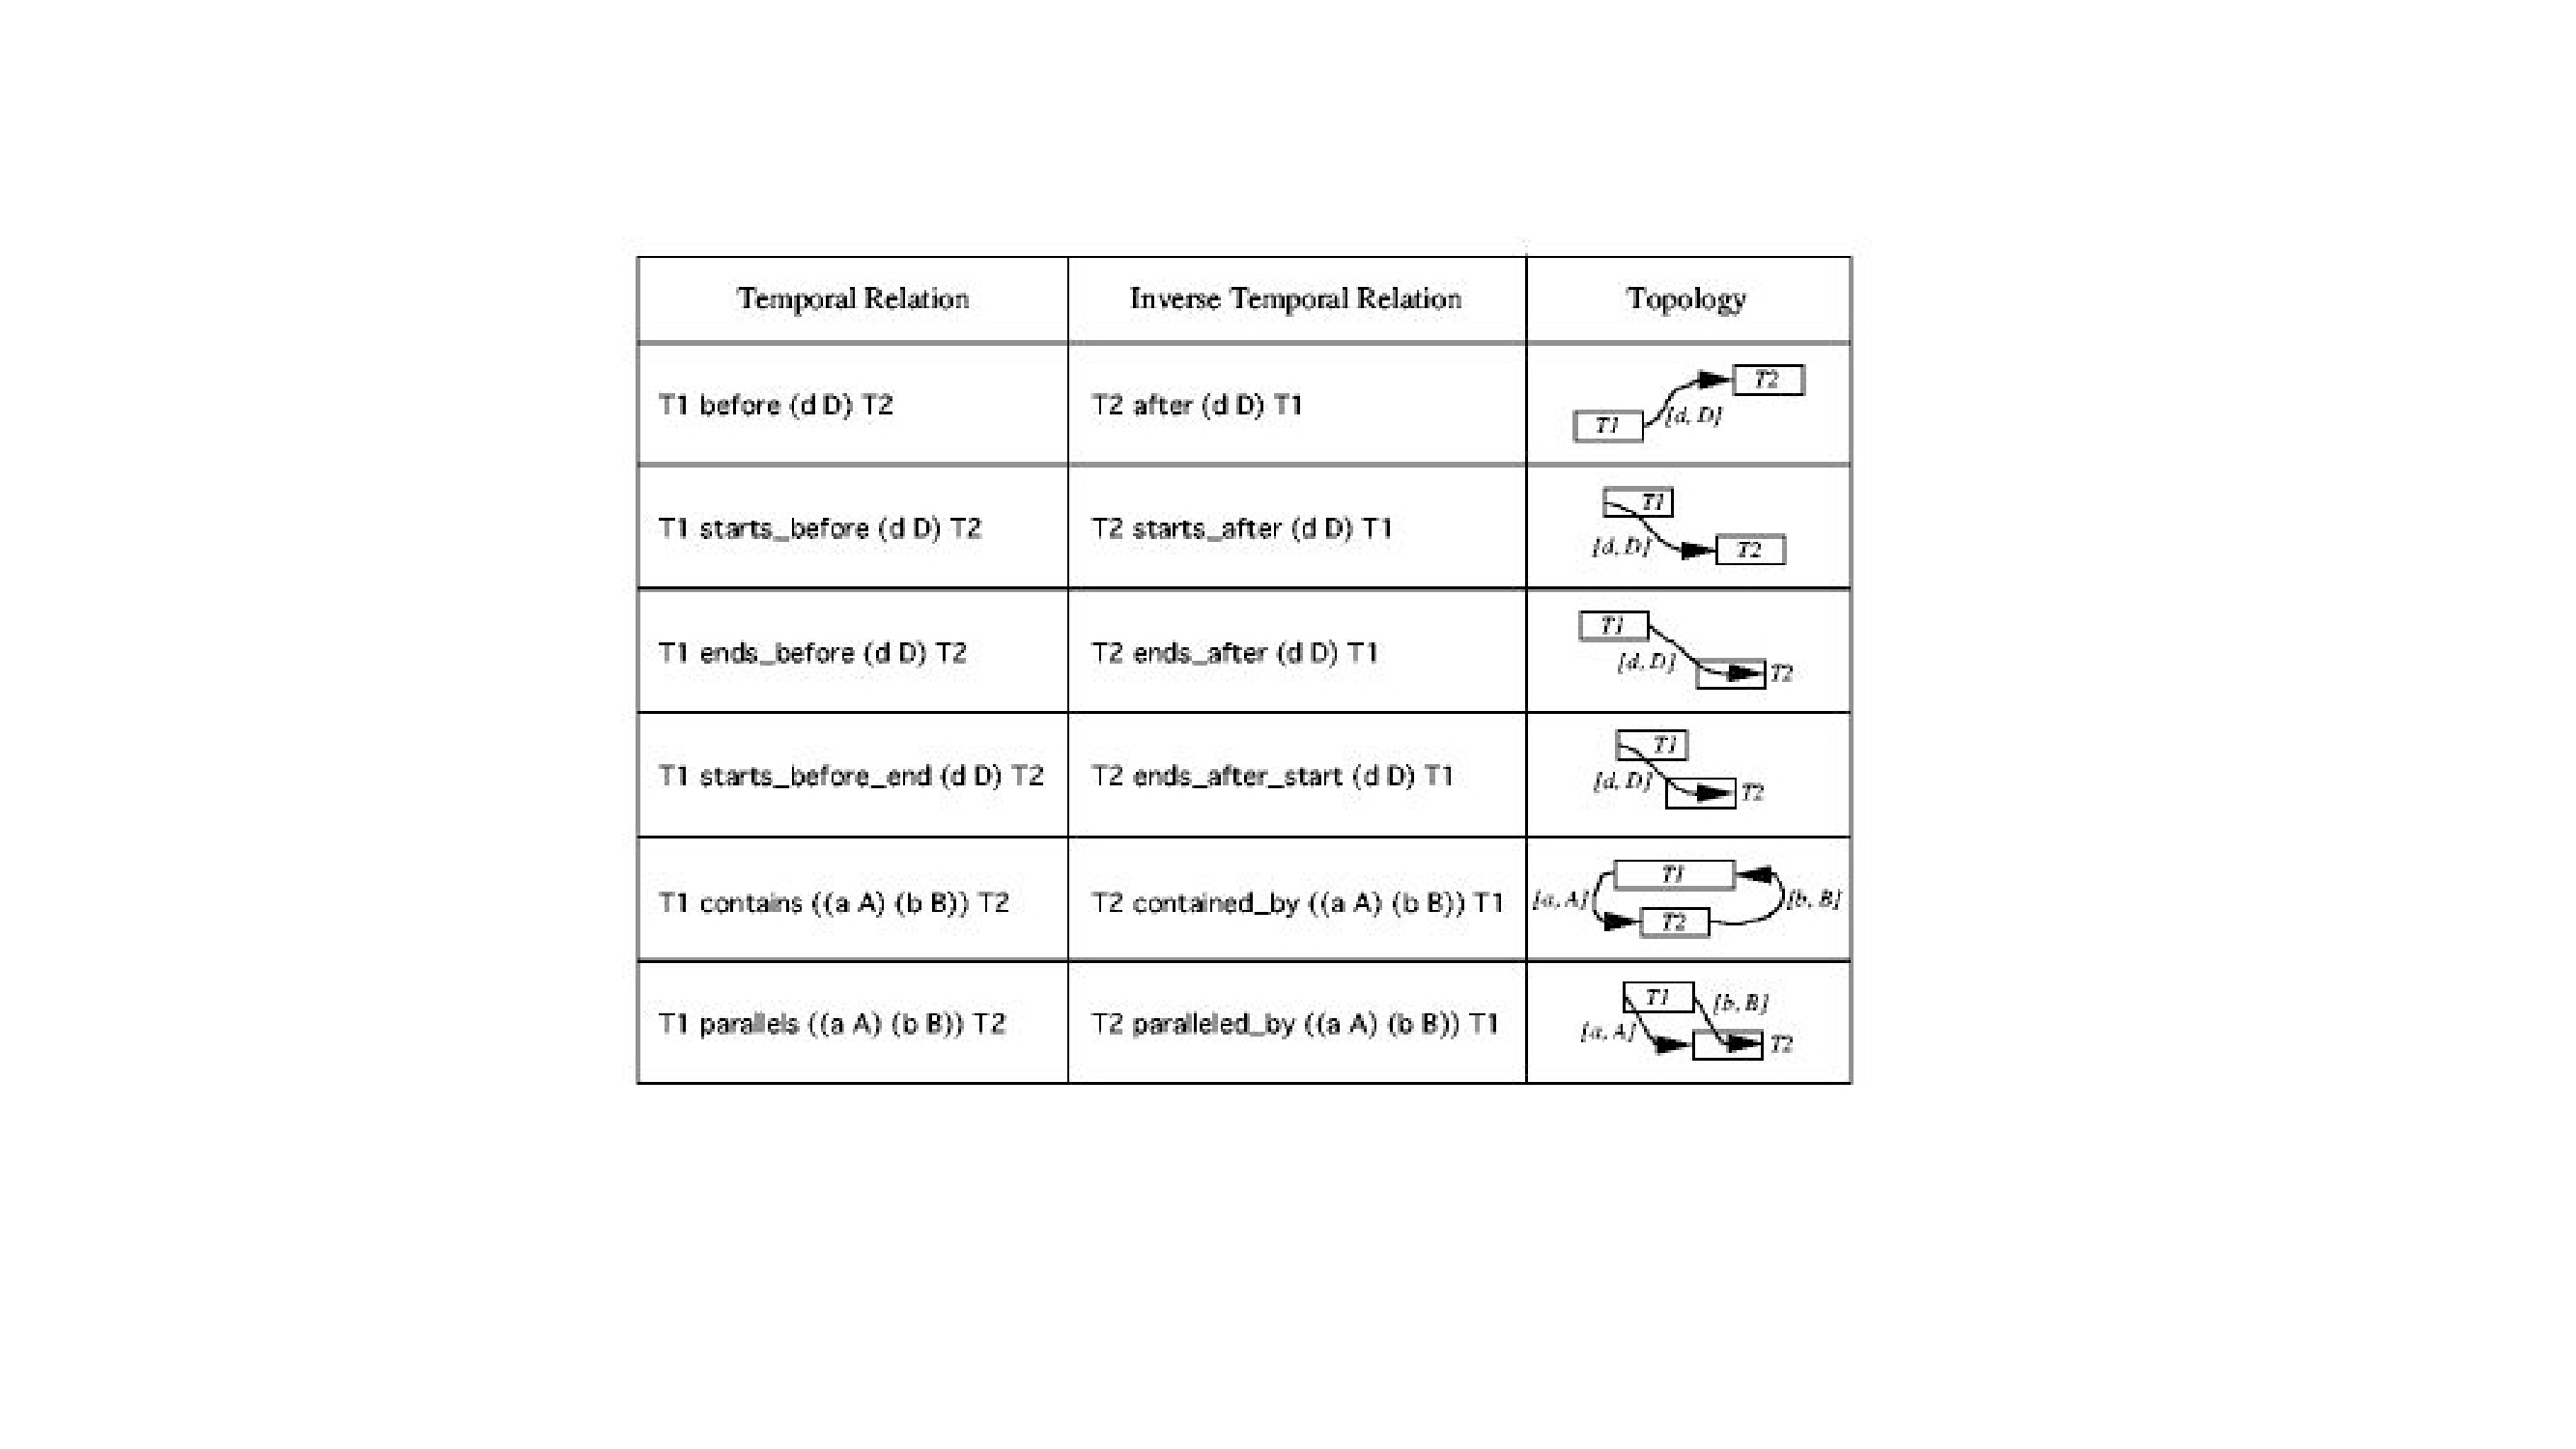
\includegraphics[scale=0.3]{figs/Allen-algebra.pdf}
\caption{\small Temporal relations defined within the planner are
  based on \texttt{Allen Algebra} relations shown above.}
\label{fig:allen-algebra}
\vskip-0.3cm
\end{figure}

\subsubsection{\eu Plan Representation}
\label{sec:europa:pr}

This section describes the fundamental entities within \eu which are
typical to other CAIP-based formalisms.

\begin{description}

\item[\textbf{Variables}] Values that need to be represented to
  describe the problem domain and over which we may want to specify
  constraints. In the Shopping Agent example, the times at which the
  agent needs to leave or be back, or executes a purchase, are all
  instances where variables representing time would be used. 
  As explained in the CP section, a variable can take values from a domain. In \eu, domains are defined over a specific data type, the primitive data types supported are:
  \begin{enumerate}
    \item \textit{String}: sequences of characters, like "Red", "Spirit", etc 
    \item \textit{Boolean}: {True,False}
    \item \textit{Numeric}: integers and floats
    \item \textit{Object}: reference to an object instance
  \end {enumerate}
  Two types of variable Domains can be defined over a data type: 
  \begin{enumerate}
    \item \textit{Enumerated}: Finite sets over any data type, specified explicitly, for instance: ["Red","Yellow","Green"], [1,18,32], etc
    \item \textit{Interval}: Only for Numeric data types, they are specified by a [LowerBound,UpperBound] pair, for instance: [1,10], [5.0,100.0], etc.
  \end {enumerate}
  \eu's ability to represent and reason over numeric intervals is a very useful characteristic that allow users to create flexible plans. \comment{say more about the benefits of flexibility?}

\item[\textbf{Objects}] The items we wish to describe and refer to in
  a domain are considered Objects. As in the case with object-oriented
  analysis and design, one can seek out the nouns in any domain
  description to find likely objects. In the Shopping Agent example,
  we night consider the Agent itself, Products and Locations all to be
  objects. Objects have state and behavior. For example, a Shopping
  Agent can have:

  \begin{itemize}

  \item State: it's location, a bag that contains the products it has
    already purchased (the bag can in turn be another object), etc.

  \item Behavior: go to a location to look for a product, perform a
    purchase, return home, etc.

  \end{itemize}

  Similarly objects that have similar state and behavior can be
  described generically in terms of object types or classes. \eu
  allows the definition of object classes in the same way that it is
  done in popular object-oriented programming languages. However, to
  describe state and behavior for the purposes of planning we need to
  build on the formalism of first order logic as explained below.

\item[\textbf{Tokens}] In first order logic, a predicate defines a
  relation between objects and properties \comment{citation?}.  In
  \eu, we define such relations between variables whose domains are
  sets of objects and sets of properties to describe state and
  behavior. For example, we might use a predicate \texttt{At($a$,$l$)}
  to indicate that agent $a$ is at location $l$, or a predicate
  \texttt{Buy($a$,$p$}) to indicate that agent $a$ is taking acting to
  buy product $p$. Note that $a$ is a variable which may have a number
  of possible values in a problem with multiple agents. Similarly, $l$
  and $p$ are variables whose values are the set of possible positions
  and products respectively. \eu can be used to create partial plans,
  where the domains of variables $a$ and $l$ can have more than one
  possible value in them, or grounded plans, where single values will
  be specified for each variable as we saw in the case of the
  N-queen's problem.

  In general, to come up with an executable plan it is not sufficient
  to state predicates that describe required state or behavior without
  also specifying some temporal extent over which each of those
  predicates hold. Predicates that are always true can be thought to
  hold from the beginning to the end of time. However, in practice,
  the temporal extent of interest must be defined with timepoints to
  represent its start and end. So we might want to write
  \texttt{At($a$,$s$,$e$,$l$)} to indicate that the agent $a$ is at
  location $p$ from time $s$ to time $e$. In fact, this pattern of
  using such predicates to describe both state and behavior of objects
  is so prevalent in \eu that we have introduced a special construct
  called a Token which has the built in variables to indicate the
  object to which the statement principally applies and the timepoints
  over which it holds. A Token is an instance of a predicate that
  represents and object's state or behavior and is defined over a
  temporal extent. In \eu, all predicate instances are Tokens. Also,
  in the same way that objects are described generically by classes,
  in \eu Tokens can be described generically by Token Types. Every
  token has five built-in variables:

  \begin{enumerate}

  \item \textit {start}: The beginning of the temporal extent over
    which the predicate is defined.

  \item \textit {end}: The end of the temporal extent over which the
    predicate is defined.

  \item \textit {duration}: The constraint \textit{start} $+$
    \textit{duration} = \textit{end} is enforced automatically.

  \item \textit{object}: The set of objects to which a token might
    apply. In a grounded plan each Token applies to a specific Object,
    reflecting the intuition that we are using Tokens to describe some
    aspect of an Object (i.e. its state or behavior) in time. However,
    in a partial plan, the commitment to a specific object may not yet
    have been made.

  \item \textit{state}: Tokens can be \texttt{ACTIVE, INACTIVE,
      MERGED}, or \texttt{REJECTED}. The state variable captures the
    token's current state and its reachable states through further
    restriction.  This is \eu's mechanism to support the CAIP approach.

  \end{enumerate}

\item[\textbf{Built-in Object Types}] In a domain model, there may be some classes that don't have any time-dependent state or behavior, and therefore those classes will not have any Token types associated with them, for instance in the Shopping Agent model, the set locations and products are static for the agent's purposes so we may only want to say what they are but not have any state or behavior associated with them.

However, the most common case in any non-trivial domain model is that Objects will have many Tokens  in order to describe their state and behavior throughout a plan. There are a couple of Object Types that are so commonly used in domain descriptions, that \eu provides a built-in implementation for them:

\begin{enumerate}
    \item \textit{Timelines}: Often objects in a domain must be described by exactly one
    token for every given timepoint in the plan. \eu provides a built-in Timeline class, any instances of a class derived from a
    Timeline will induce ordering requirements among its tokens in order
     to ensure no temporal overlap may occur among them  \cite{mus94}. 
     \comment{add small example?}

    \item \textit{Resources}: Metric resources, e.g. the energy of a battery or the
    capacity of a cargo hold, are objects with an explicit quantitative
    state in time and with a circumscribed range of changes that can occur
     to impact that state i.e. produce, consume, use, change. 
     Resources are such a common requirement for \eu users that built-in object types (with their corresponding token types to denote production, consumption, etc) are provided for them. Instances of classes derived from a Resource will induce
     ordering requirements on their Tokens in order to ensure that the
     level of the resource remains within specified limits.
     \comment{add small example?}
\end{enumerate}

\comment {resume cleanup here}

\item[\textbf{Token State Model}] The capability of a domain rule to cause a slave token to be created
is a key vehicle through which planning occurs. Semantically, this
rule imposes a requirement for supporting tokens to be in the plan in
order for the master to be valid. There are 2 possibilities to
consider:

The slave is inserted as an active token in the plan. As such, rules
may be activated on the slave, and it may consume resources.

The token is merged with a matching token already in the plan. Once a
slave is merged, the requirement it represents are considered
satisfied. The process of merging passes on all restrictions imposed
on the slave to the active token upon which it is merged. Merging a
token requires finding a target active token that is compatible with
the inactive token. For an active token and an inactive token to be
compatible requires that they are instances of the same predicate and
that no intersections between corresponding variables are empty. The
effect of merging is illustrated in Figure 3.

Figure 3: Merging an inactive token on an active token. Domain
restrictions occur in highlighted variables of active token.

On creation of a token, where the commitment has not been made yet to
activate or merge the token, the token is said to be inactive. There
is a nuance to the state model for tokens which relate to the mode of
its creation. If the token is allocated explicitly by an external
actor, rather than internally through rule firing, it may include the
state rejected indicating the planner is permitted to reject the
token. A valid plan can include rejected tokens. This typically arises
where the token represents a goal that is preferable to achieve but
not mandatory. This state is not reachable for slaves since that would
imply selective adherence to the domain model. Figure 4 presents the
state transition diagram for token states relevant for planning. The
transitions are operations on a partial plan which can decide an
outcome for an inactive token. As operations which may arise in
search, they must be reversible during backtracking. The cancellation
operations in each case are also shown.

\item[\textbf{Rules}] In order for a plan to be valid, it must comply with all rules and
regulations pertinent to the application domain in question. Rules
govern the internal and external relationships of a token. For
example, consider a parameterized predicate describing a transition
from one location to another. Let the parameters be from and to. The
parameters are instantiated on a token as variables whose domain of
values is the set of all locations in a given problem. A rule
governing an internal relationship among token variables might
stipulate that a transition must involve a change in location. This
can be easily expressed as a constraint on the definition of a
predicate of the form: from != to. It is reasonable to further
stipulate that one must be Located somewhere before a transition can
occur, and one must end up Located somewhere when completed. This is
an example of a rule governing an external relationship among
tokens. It specifies a requirement that tokens of the predicate
Located precede and succeed tokens of the predicate Moving.

Figure 2: Internal and external relationships from rules on Moving
Figure 2 illustrates the entities and relations involved in specifying
such a rule on a Moving predicate. The token on which the rule applies
is referred to as the master. Each Located token required by the
master is referred to as a slave. All variables are indicated by name
and their domains are expressed as intervals in the case of temporal
variables and as enumerations for the remainder. Application of a rule
on a token can thus cause slave tokens, variables, and constraints to
be introduced.  

\end{description}

\comment{instead of summary, tie every concept to the shopping example?}

This section has presented the main elements of \eu's planning representation:

\begin{enumerate}
    \item Temporally scoped predicates and actions (a.k.a. Tokens) to represent
    states and actions in time. Note that tokens do not discriminate between state and action. 

    \item Token States which are the basis of planning operations on a partial plan.

    \item Constraints to describe relationships among tokens. This provides an
    expressive method of describing interactions among tokens in the context of Temporal Planning.

    \item Timelines as a concise abstraction to express the evolution of state
    and behavior for a system component. It provides semantics of mutual
    exclusion sequencing in time. Other core abstractions are available in
    \eu for handling metric resources.

    \item Domain rules to describe internal and external relationships on and
     between tokens respectively. Rules are applied to active tokens (master tokens) 
     referred to as masters and typically produce inactive
     tokens (slaves) which are a key vehicle through which the planning
     process evolves. The rule structure in \eu differs from the more
     restrictive commitment to preconditions and effects in classical
     planning which prohibits durative actions and disembodied effects
     (i.e. effects which may not occur until some temporal distance after
     the end of the action).
\end{enumerate}

 
%Each of the token variables, including the parameter variables, has a
%domain of values assigned to it.  The variables may also participate
%in constraints that specify which value combinations are valid.  To
%allow the specification of multiple values, e.g, to express a range of
%possible start times, variables are used to specify parameter, start
%and end time values for a token.  As a result, a token $T$ is a tuple
%$\langle v, P, s, e \rangle$, where $v$ is a variable denoting a state
%variable, $P$ is the name of a procedure and $s$ and $e$ (satisfying
%$s\leq e$) are variables encoded as flexible token start and end time
%points. Consequently, partial plans represent a \textit{range of
%  possible solutions} rather than an explicit definition of a single
%trajectory of state.  Fig. \ref{fig:flex-timelines} shows an example
%of a part of such plans with tokens representing constraints on
%flexible temporal intervals. Systematic computation is reflected by
%the use of the \texttt{Allen Algebra} \cite{allen84} temporal
%relations shown in Fig. \ref{fig:allen-algebra}. It is the use of such
%interval arithmetic in the \eu domain model that allows
%encoding of temporal constraint relationships between tokens on the
%same or other concurrent timelines. Details of propagation algorithms
%or of interval logic are beyond the scope of this paper.
%
%\begin{figure}
%\centering
%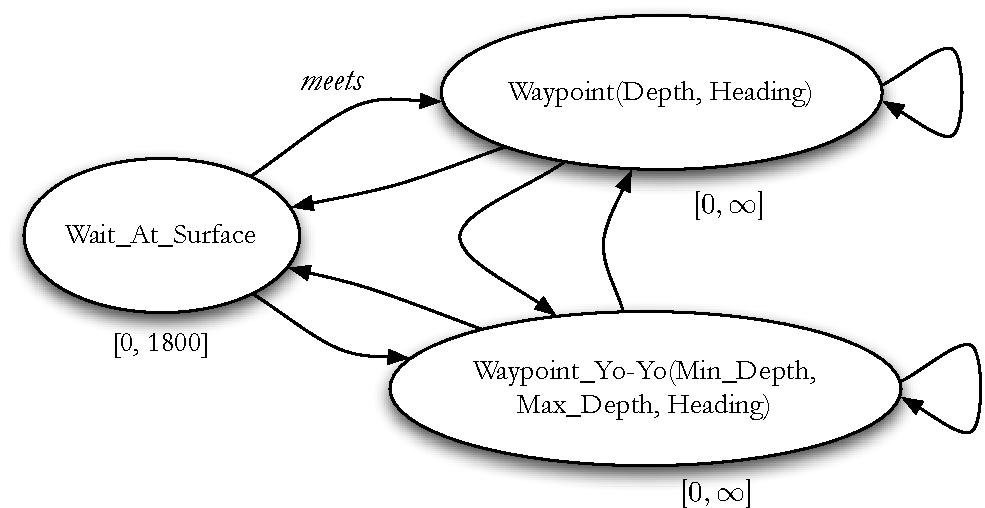
\includegraphics[scale=0.3]{figs/FSM-transition.pdf}
%\caption{\small Timeline evolution can be described by simple finite
%  state transitions where temporal relationships describe the arc
%  transition and temporal extant of state are token
%  durations. Constraints here are for \emph{meets} or its equivalent
%  inverse \emph{met\_by}.}
%\label{fig:FSM}
%\vskip-0.3cm
%\end{figure}
%
%In describing the evolution of state via timelines, transitions within
%a timeline can be described by simple finite state
%machines. Fig. \ref{fig:FSM} for example describes a timeline
%evolution for an abstract timeline entity describing navigation. Arc
%transitions represent temporal constraints and token duration are
%represented by temporal extant of state. The entire vehicle can then
%be modeled as a number of state transitions with concurrency for each
%of the modeled state variables defined a priori. However this simple
%view is often complicated when temporal constraints between state
%variables are articulated in our domain models. If there is a
%criticism of this approach, modeling then, requires a proper balance
%between abstraction, state variable description and concurrency
%described by the inter-connectedness between such finite state
%machines.

%For example, consider the tire-world domain. The tire was located in
%the trunk with the predicate tireLocated(Trunk) and located on the
%ground with the predicate tireLocated(Ground). Clearly, the same tire
%cannot be in both places at once. A Timeline provides a simple method
%for aggregating the statements about a tire such that they are
%mutually exclusive.
%
%Figure 1: A Timeline for a Tire
%
%Figure 1 illustrates how a Timeline can be used to describe the
%whereabouts of a tire. The tire is an object in the tire-world
%represented as a timeline. It has predicates associated with it which
%can describe its states and actions over time. The predicate names
%need not contain the tire prefix; this is now implicit since the
%tokens are assigned to a specific tire instance (i.e. an instance of a
%Timeline). While Timelines are a useful element of the \eu planning
%paradigm, they are not essential. A more general notion of a system
%Object can be used which does not impose restrictions of
%mutual-exclusion or non-zero duration. This can be important in
%supporting partial-order planning.
%
%For this example, the state of the tire is specified using 3
%contiguous tokens. The end and start time-points are related by an
%equality constraint. A Moving predicate has been introduced to cover
%the transition from one location to another. It takes 2 location
%arguments. Notice that precedence relationships exist between tokens
%such that they cannot overlap but the start and end times may remain
%flexible. To illustrate this, sample times are included. Assume a
%total time range of interest between 0 and 1000. In addition, tokens
%on Timelines have a minimum duration of 1. As a result the values
%shown are the most flexible possible values for the start and end of
%each token. There are a number of advantages of allowing this
%flexibility. First, the basic structure of the plan can be developed
%without over-committing to specific times. If it is not necessary for
%the tire to be on the ground at time-step 4, then a planner should not
%be forced to specify it. Such an approach permits a least-commitment
%approach to planning. Second, in many domains it is simply impossible
%to know in planning exactly how long an activity might take. For
%example, a common activity of driving a car from one point to another
%on a road can take varying amounts of time depending on traffic and
%traffic lights. In such circumstances it is more practical to express
%upper and lower bounds on durations which naturally lead to intervals
%for start and end times. In such domains, flexibility in planning aids
%robustness in execution.  


\begin{figure*}
\centering 
\subfloat[]{\label{fig:plan-evolve1}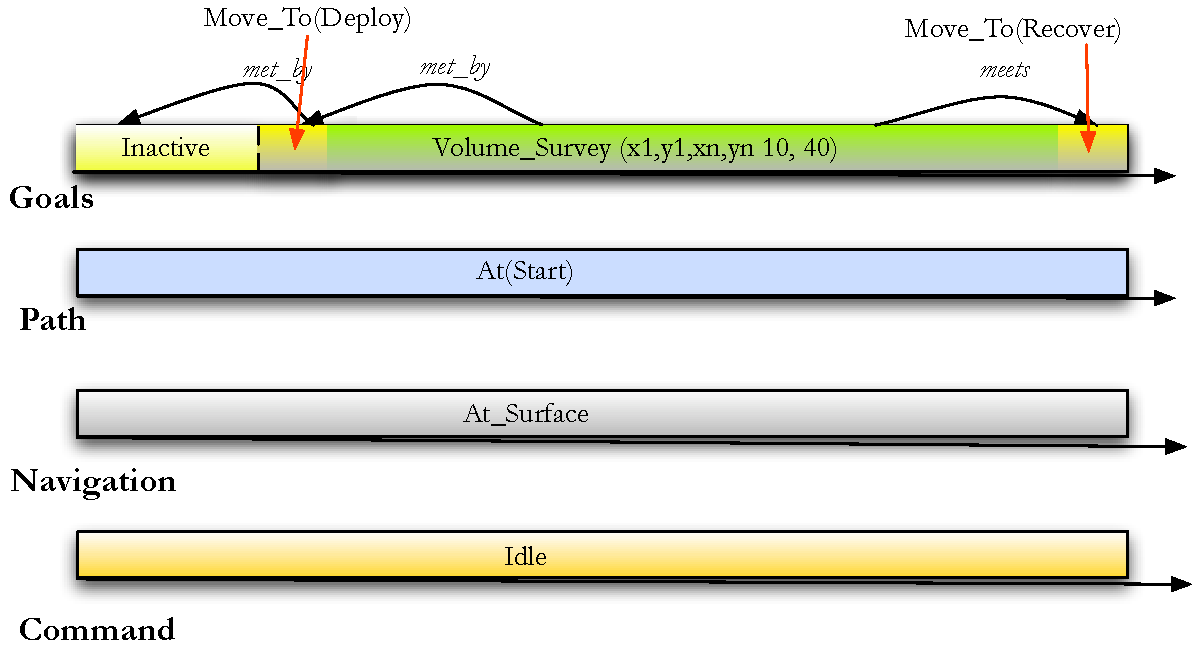
\includegraphics[width=0.3\textwidth]{figs/Plan-evolve-1.pdf}} 
\subfloat[]{\label{fig:plan-evolve2}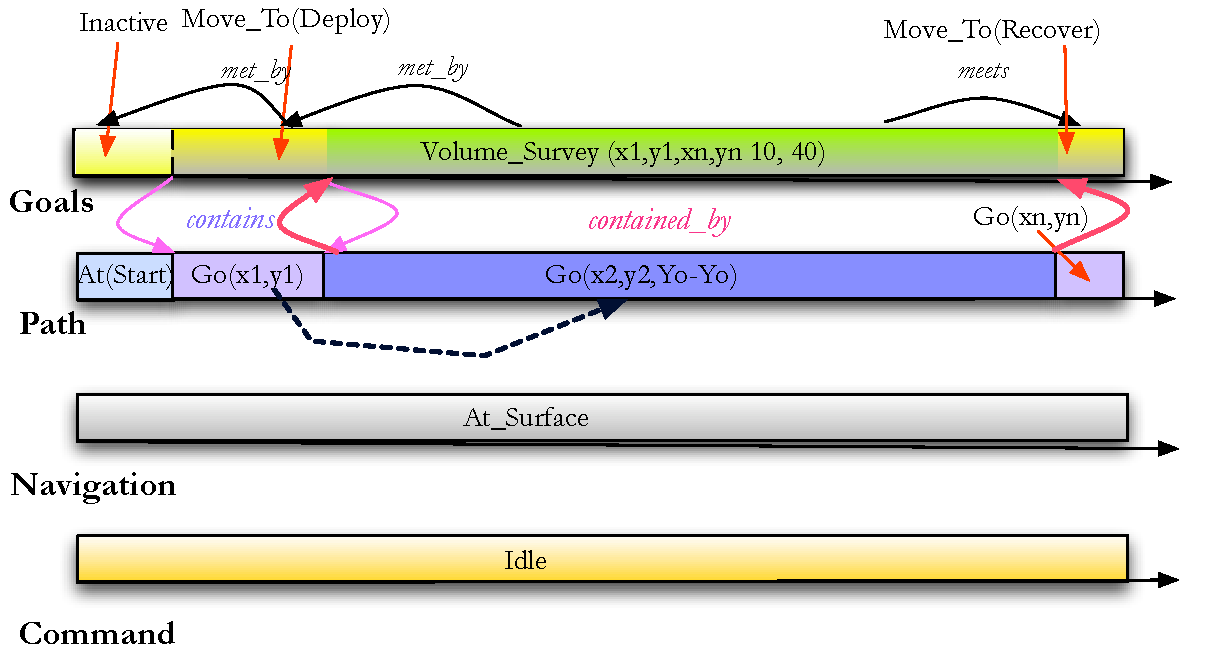
\includegraphics[width=0.3\textwidth]{figs/Plan-evolve-2.pdf}} 
\subfloat[]{\label{fig:plan-evolve3}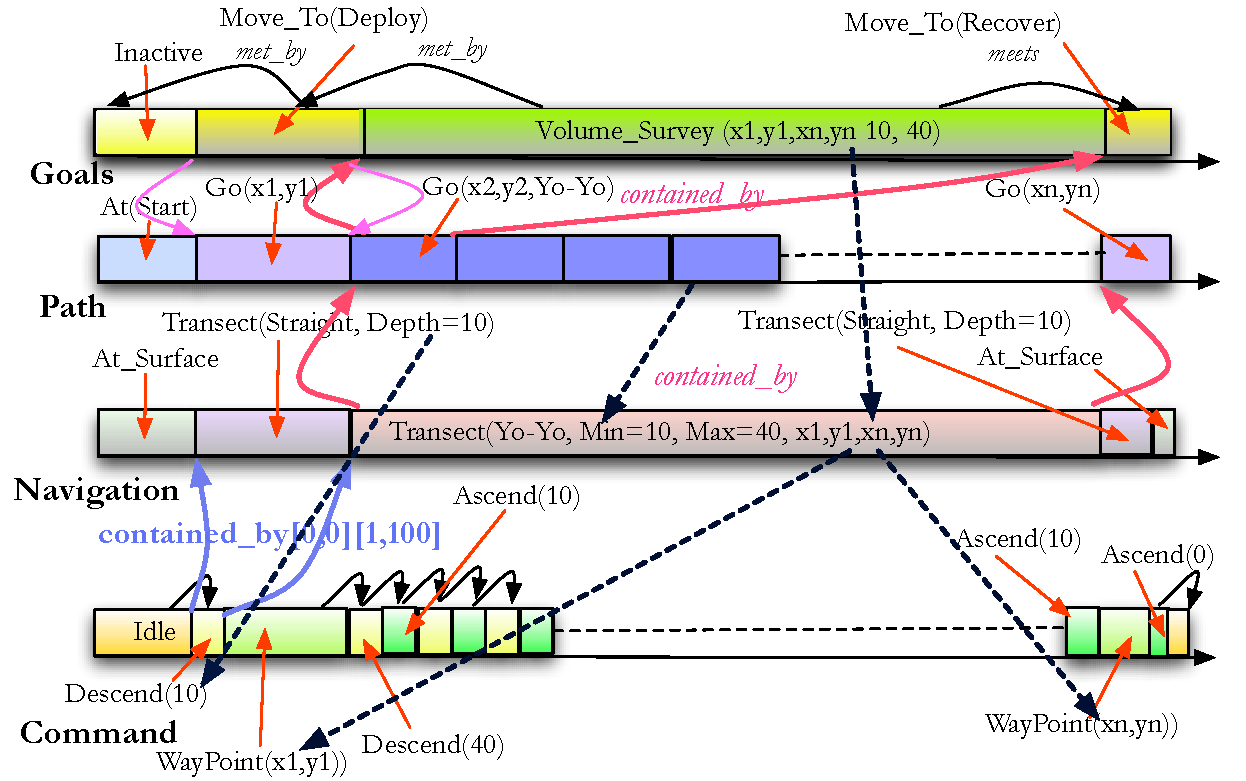
\includegraphics[width=0.3\textwidth]{figs/Plan-evolve-3.pdf}} 
\caption{\small An illustrative plan synthesis example with concurrent
  timelines. Each timeline is an instantiation of a subsystem tracked
  by the planner. Tokens describe the instantiated state of subsystem
  at a particular time instance and enforce temporal and parametric
  constraints. Abstract goals are decomoposed into successively less
  abstract tokens and instantiated in co-temporal timelines using
  \texttt{Allen Algebra} relations. All tokens represent flexible
  start/end times. \ref{fig:plan-evolve1} shows an initial state
  evolving into \ref{fig:plan-evolve2} and \ref{fig:plan-evolve3}.}
  \label{fig:Plan-evolve}
  \vskip-5pt
\end{figure*}

Fig. \ref{fig:Plan-evolve} shows an illustrative example. We show four
timelines which track \texttt{Goal, Path, Navigation} and
\texttt{Command} state over time. Tokens on the goal timeline indicate
a survey within a bounded volume and a min/max depth envelope. As the
Volume Survey sub-goals on the \texttt{Path} timeline, the initial
token on that timeline gets \emph{squeezed} to have dependencies of
the goal token instantiated. Initially this dependency are the tokens
\texttt{Go(x1,y1)} and \texttt{Go(xn,yn)} indicative of the area of
coverage. The first of these in turn generates a sub-goal on the same
timeline to go to the next intermediate waypoint, which is illustrated
in Fig. \ref{fig:plan-evolve2}. Subsequent sub-goals (not shown in the
figure) ultimately generate all the tokens to completion for this
timeline. Fig. \ref {fig:plan-evolve3} shows a snapshot further along
in plan generation and shows additional subgoals on the \texttt{Path,
  Navigation} and \texttt{Command} timelines. Each token can thus
trace its causality when instantiated in the plan. The domain model
provides source of these temporal and parametric dependencies in the
form of rules. 


\begin{minipage}[c]{\textwidth}
\vspace{+0.5cm}
% \framebox[\textwidth][t]{
Volume\_Survey(x$_1$,y$_1$,x$_n$,y$_n$,Min\_Depth, Max\_Depth)\\
$\Rightarrow$ \\
met\_by Go(x$_1$,y$_1$,Min\_Depth); \\
starts [50,0] Go(x$_2$,y$_2$,Min\_Depth,Max\_Depth); \\
\ldots{} \\
ends [50,0] Go(x$_{n-1}$,y$_{n-1}$, Min\_Depth,Max\_Depth); \\
meets Go(x$_n$,y$_n$,Min\_Depth, Max\_Depth); 
\end{minipage}

% \end{enumerate}



% \subsubsection{Partitioned Control}


% \subsubsection{State Estimation}

% Even as automated reasoning approaches have the ability to dynamically
% retarget the vehicle, estimating environmental signals of interest (or
% their proxies) is important to be able to enable opportunistic science
% in the water-column. In \texttt{T-REX} feature recognition revolves
% around a Hidden Markov Model (HMM) \cite{rabiner86} which is encoded
% directly within the unified representational and computational
% framework of a reactor. HMMs are useful since the stochastic nature of
% these models can correlate the type of features we want to detect with
% the sensor observations. Online targeted sensor data is classified by
% apriori generated cluster data which in turn determines the
% probability of having seen the feature of interest. Together with
% posterior probability, the HMM generates a probability of being within
% the target feature if it dominates the distribution. If other sampling
% conditions are satisfied (for instance sampling proximity), a
% constraint is activited in the model which can trigger a water sampler
% and also preserve the memory of sampling to alter a future transect
% resolution.


% The HMM is customized for the feature of interest and is built offline
% using clustering techniques from large data sets; we use Kohonen's
% Self Organizing Maps \cite{kohonen}. We use a semi-supervised learning
% method \cite{zhu05} to extract an environmental model that make uses
% of both labeled and unlabeled data for training. Online,

% The sensor data for classification depends on the
% feature of interest; for detecting INLs we use backscattering data
% from a HydroScat and for tracking riverine plumes to track fertilizer
% runoff, we use an ISUS Nitrate sensor.

%%% Local Variables: 
%%% mode: latex
%%% TeX-master: "ieee-ram09"
%%% End: 
